\documentclass[10pt]{article}
\usepackage{epsf}
\usepackage{amsmath}
\usepackage{amssymb}
\usepackage{palatino}
\usepackage[pdftex]{graphics}
\usepackage{fancyhdr}
\usepackage{epsfig}
\usepackage{multirow}
\usepackage{multicol}
\usepackage{cancel}
\usepackage{hyperref}
\usepackage{longtable}
\usepackage{ulem}
\usepackage[yyyymmdd]{datetime}
\renewcommand{\dateseparator}{-}
\usepackage{listings}

\parindent 0in
\parskip 1ex
\oddsidemargin  0in
\evensidemargin 0in
\textheight 8.5in
\textwidth 6.5in
\topmargin -0.25in

\pagestyle{fancy}
\lhead{\textbf{\leftheader}}
\rhead{\textbf{\rightheader}}
\lfoot{Compiled: \today\ \currenttime}
\cfoot{}
\rfoot{\thepage}

\newcommand{\leftheader}{BME290L: MedTech Prototyping Skills}
\newcommand{\rightheader}{Palmeri (Spring 2023)}

\begin{document}

\title{Lab 07: Blinking Light Enclosure} 
\author{MedTech Prototyping Skills (BME290L)}
\maketitle

\textbf{Before you start this lab exercise--and because Sakai Drop Box
stinks--please upload the zip archive of your KiCad Project for Lab 06 to Box
(\href{https://duke.box.com/s/e0xdfqhgh0933gnydfww605tubeysxft}{Lab06-PCB-Layout}).\\\\
Please make sure that your zip filename is: LastnameFirstName\_v3.x.x.zip
(e.g., PalmeriMark\_v3.0.0.zip).}
\section{Design: Sketch}
\subsection{External Design}
On paper (or electronic sketch), design an enclosure for your blinking light
device that satisfies the following specifications:
\begin{itemize}
    \item Ergonically held in one hand
    \item Ability to ``easily'' push the button to turn on the blinking lights
        with the hand holding the device
    \item Can be stable placed on a flat surface and operated without picking it up from that flat surface.
    \item Batteries can be ``easily'' replaced.
    \item Power switch will not be inadvertantly switched "off" during operation.
    \item Potentiometer knobs are accessible, but can use a second hand to
        adjust them.
\end{itemize}

\subsection{Internal Design}
Consider the following internal design criteria:
\begin{itemize}
    \item Board is securely mounted using your 4 mounting holes.
    \item Test pads will be accessible for testing the electronics when the
        board is mounted inside (assuming a cover of some sort can be removed
        to access the board).  In other words, the entire board does not need
        to be removed for any debugging / testing.
    \item Wires between the PCB connectors and the peripheral components are
        purposely routed / secured internally.
    \item All peripheral components securely mounted in outer shell of the
        enclosure.\footnote{Exact components available will be specified on
        Thursday.  For now, represent with 5 mm holes, 10 mm diameter part
        width internally with 10 mm of internal depth clearance from the inner
        shell surface.}
    \item Batteries securely mounted using 2x2 or 1x4 AA battery holders.
\end{itemize}

\section{Things to Optimize}
\begin{itemize}
    \item Size (smaller is better)
    \item Weight (again, smaller is better)
    \item Weight balance ("hand feel")
    \item Ergonomics / aesthetics.  Try to avoid corners and straigh edges.
        Curves are good (and not sharp).
    \item Stress concentrations if your device fell from 6 ft.
\end{itemize}

\section{Modify your PCB Layout}
Most folks will have some epiphanies during the enclosure design that will be
best served by modifying your PCB layout.  Please do this, and reflect these
changes with an increment in the minor revision number of the PCB layout (not
the schematic, unless you also make changes to that).

\section{Design: CAD}
\subsection{Utilizing your sketch in Onshape}
\begin{itemize}
    \item Import useful sketch planes into Onshape as a template for starting your sketches.
    \begin{itemize}
        \item \url{https://cad.onshape.com/help/Content/sketch-image.htm}
        \item Import Image\\
        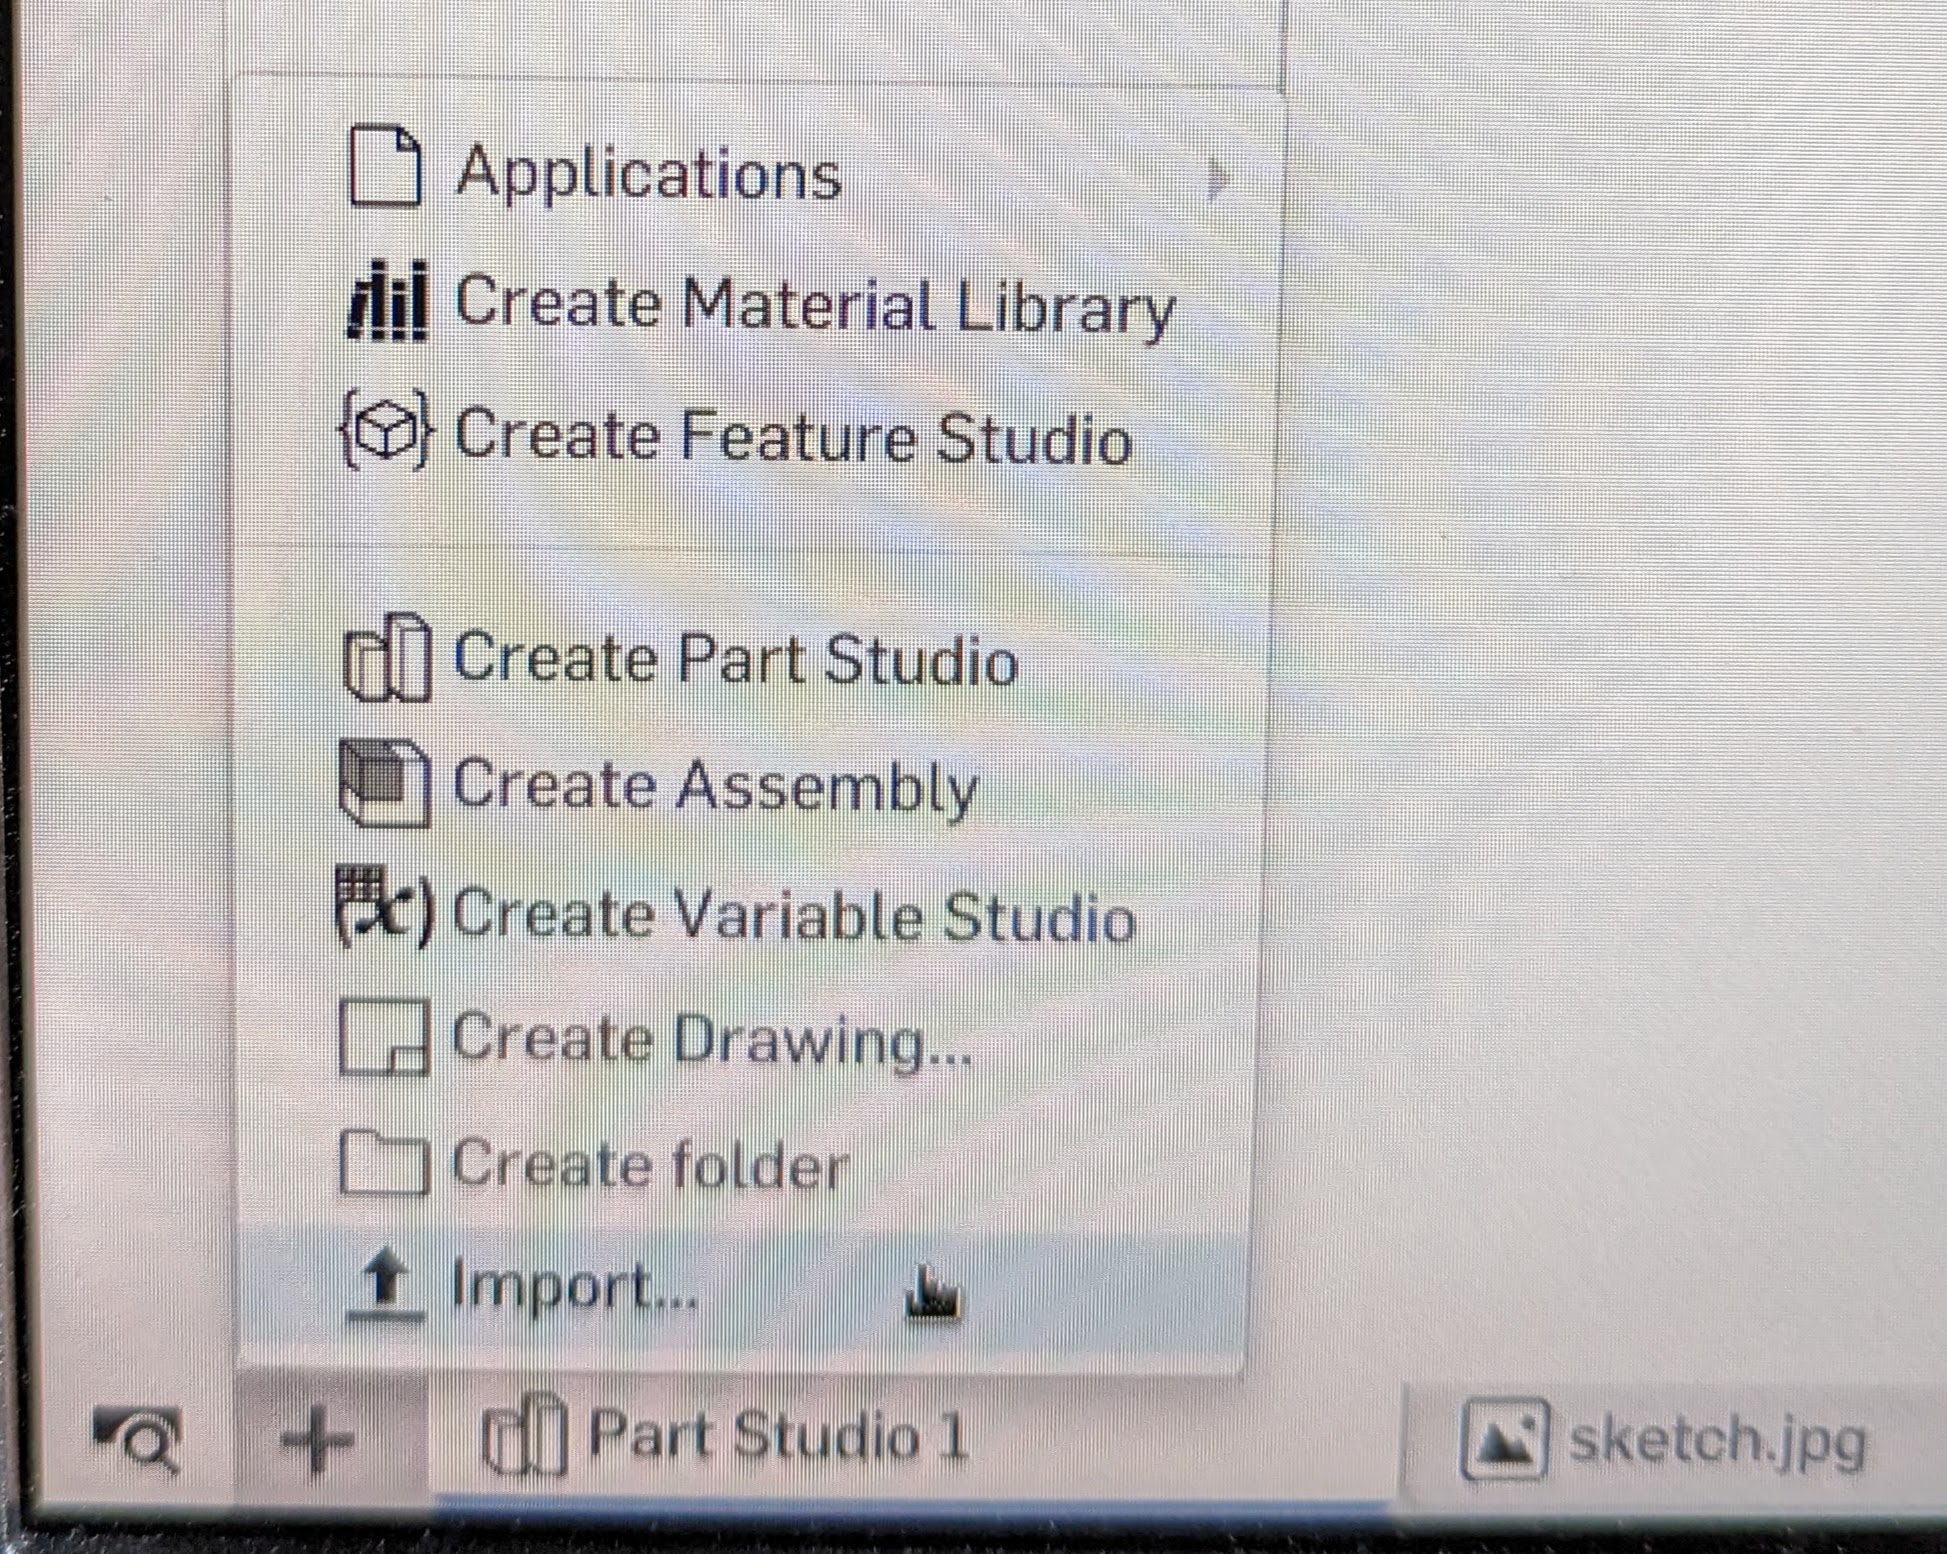
\includegraphics[width=0.5\textwidth]{import_image.jpg}
        \item Insert Image in sketch (after selecting sketch plane)\\
        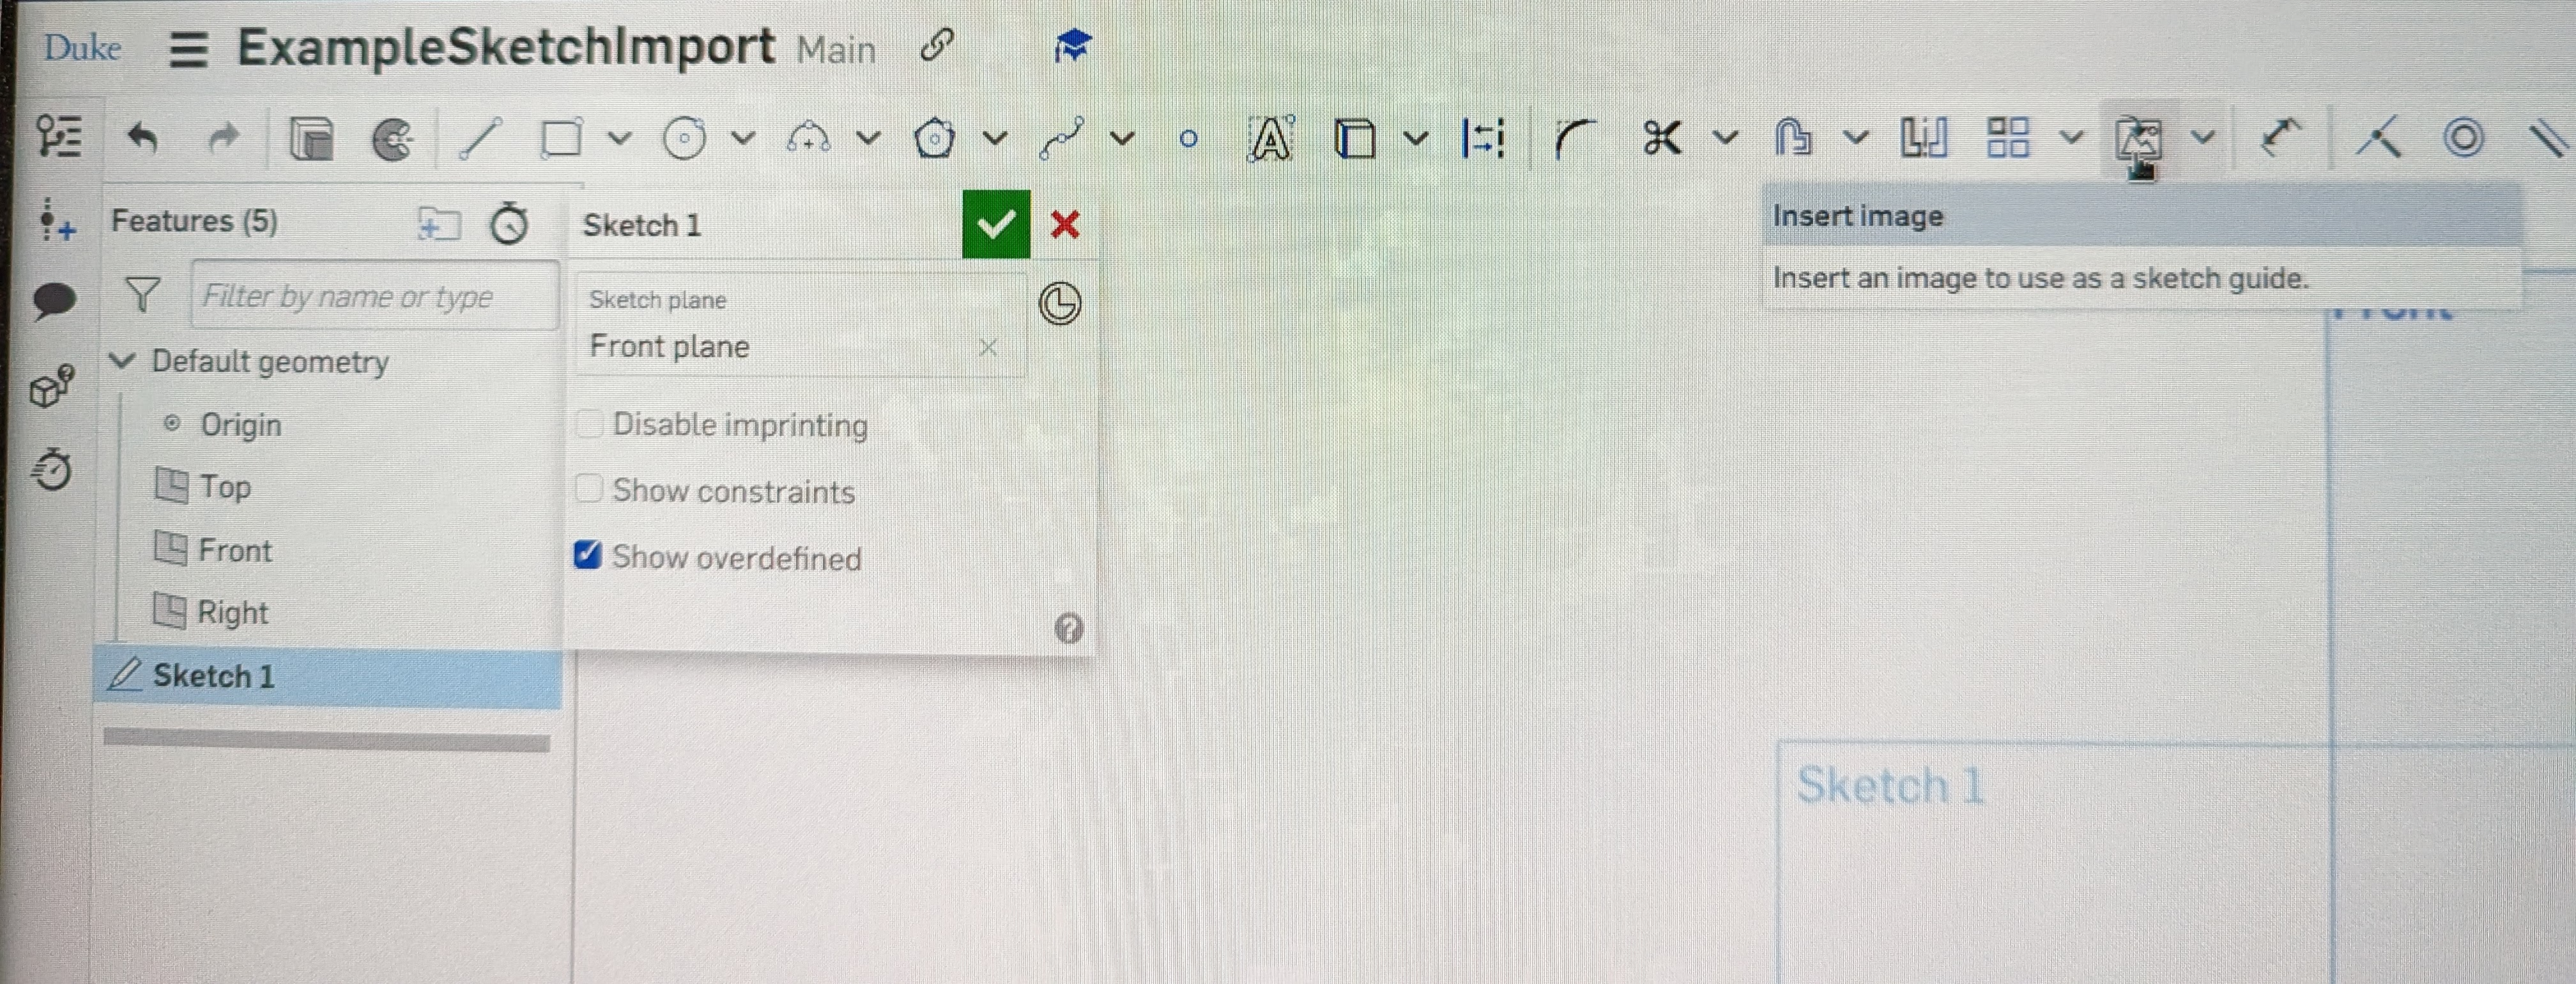
\includegraphics[width=0.5\textwidth]{insert_image.jpg}
        \item Rotate / center / scale image(s) to align with where you want to sketch.
        \item Mirror the sketch (in the sketch!) to avoid asymmetry.
    \end{itemize}
    
Example: \url{https://duke.onshape.com/documents/9495fbc8174cd66096d0184b/w/2e71fa76452c602f94cf4afc/e/dd5c3b6e6248d71fa8073ad5?renderMode=1&uiState=63f4d823a80f864f4cf5bcd4}\\
\centerline{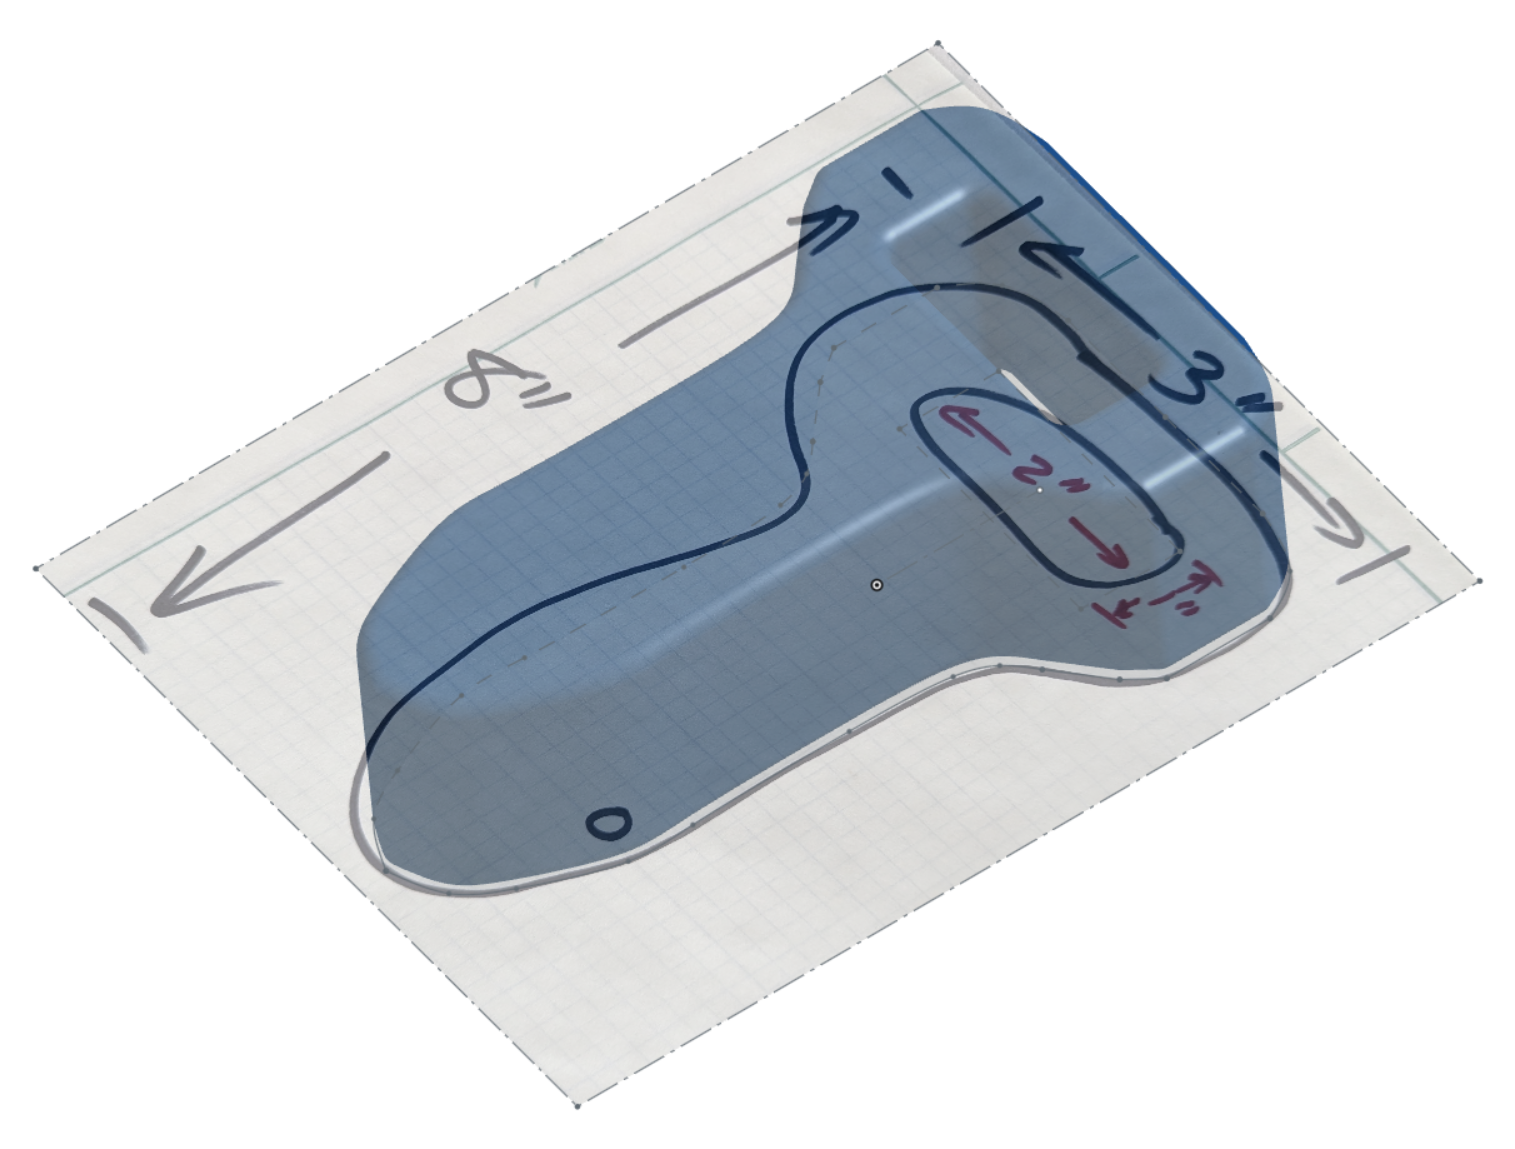
\includegraphics[width=0.75\textwidth]{rendered_part_from_sketch.png}}

    \item Expand your part into 3D.
    \item Fit your PCB
    \begin{itemize}
        \item Export your PCB as a STEP file, being sure to select \texttt{Substitute similarly named models}.
        \item Import your STEP model into Onshape.
            
        \centerline{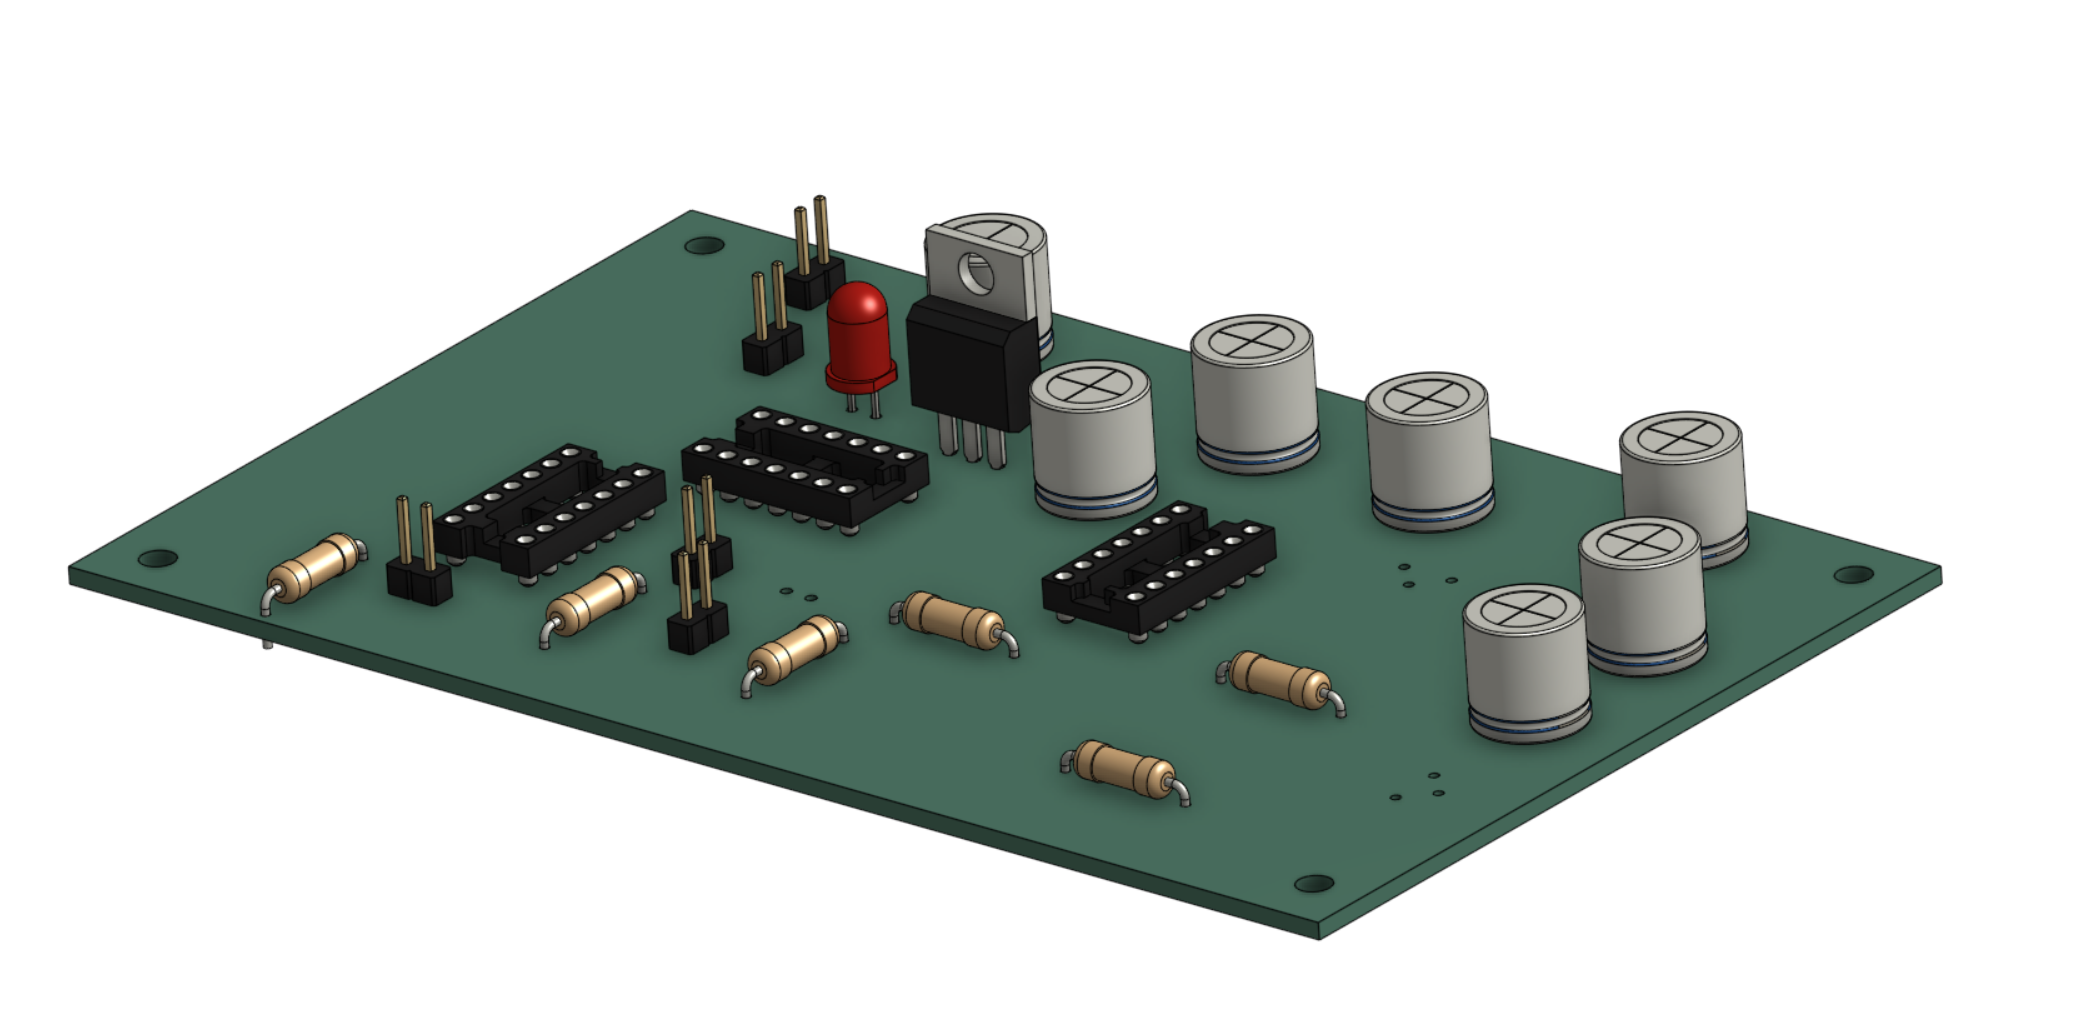
\includegraphics[width=0.8\textwidth]{pcb_step_import.png}}
    \end{itemize}
    \item "Cut" your part into pieces that are amenable to 3D printing.
    \item Assemble your PCB and enclosure.
\end{itemize}

\section{What to Submit}
\begin{enumerate}
    \item Share your Onshape project with Mark, Rebecca, Nikhita and Nikhil.
    \item Upload a PDF of your exploded assembly (3D rendering, not drawing) to Gradescope, showing all
        parts, including the PCB.
    \item Please upload a zip archive of your updated PCB (I assume almost
        everyone will want to modify their PCB layout) to Box:
        \href{https://duke.box.com/s/byhnj190aegac09hg0gdr1j1x1hux02u}{Lab07-Enclosure-PCBmods}.\\\\
        Please use the same filename convenstion as Lab 06 (e.g.,
        \texttt{PalmeriMark\_v3.1.0.zip}).\\\\If you do not make any changes to
        your PCB layout, then please just upload the same zip archive that you
        did for Lab 06.
    \item You do \emph{not} need to generate mechanical drawings with
        dimensions for your design (yet).
\end{enumerate}

\end{document}